\documentclass[a4paper, czech]{article}

\usepackage[czech]{babel}
\usepackage{indentfirst}
\usepackage{graphicx}
\usepackage{float}
\usepackage[margin=1.5cm]{geometry}
\usepackage{booktabs}
\usepackage{amsmath}
\usepackage{xcolor}
\usepackage{multirow}
\usepackage{tabularray}
\usepackage{bold-extra}

\begin{document}
\begin{table}[H]
    \centering
    \begin{tblr}{
        cell{1}{1} = {c = 2, r = 4}{c}, % Logo
        cell{1}{4} = {c = 3}{c}, % Předmět
        cell{2}{4} = {c = 3}{c}, % Jméno
        cell{3}{4} = {}{c}, % Ročník
        cell{3}{6} = {}{c}, % Studijní skupina
        cell{4}{4} = {}{c}, % Spolupracoval
        cell{4}{6} = {}{c}, % Mereno dne
        cell{5}{1} = {c = 2}{55mm}, % Kontroloval
        cell{5}{3} = {c = 2}{55mm}, % Hodnoceni
        cell{5}{5} = {c = 2}{55mm}, % Dne
        cell{6}{2} = {c = 5}{}, % Nazev ulohy
        cell{7}{1} = {}{c}, % Číslo úlohy
        cell{7}{2} = {c = 5}{c}, % Název úlohy
        vline{1,2,7} = {1.2pt},
        vline{3,5},
        hline{1,5,6,8} = {1.2pt},
        hline{2,3,4}
        }
        
\includegraphics{logo_fekt.png} & & \textsuperscript{Předmět} & \large \textbf{Měření v audiotechnice} \\
             & & \textsuperscript{Jméno} & \large \textbf{Karolína Šebestová} \\
             & & \textsuperscript{Ročník} & \large \textbf{3.} & \textsuperscript{Studijní skupina} & \large \textbf{St 14:00} \\
             & & \textsuperscript{Spolupracoval} & \large \textbf{Filip Kokavec} & \textsuperscript{Měřeno dne} & \large \textbf{2.10.2024} \\
        \textsuperscript{Kontroloval} & & \textsuperscript{Hodnocení} & & \textsuperscript{Dne} \\
        \textsuperscript{Číslo úlohy} & \textsuperscript{Název úlohy} \\
        \Large \textbf{1} & \Large \textsc{\textbf{Stanovení nejistot při nepřímém měření výkonu}} \\
    \end{tblr}
\end{table}

\section{Zadání}

\begin{itemize}
    \item Seznamte se s měřením stejnosměrného proudu a napětí pomocí ČMP a s určením nejistoty nepřímého měření výkonu.
    \item Změřte výkon stejnosměrného proudu nepřímou metodou.
    \item Naměřené hodnoty zpracujte z hlediska odchylky metody a nejistot měření.
\end{itemize}

\section{Teoretický úvod}

Výkon stejnosměrného obvodu lze jednoduše měřit nepřímou metodou, kdy nejprve měříme elektrické napětí voltmetrem a elektrický proud ampérmetrem.
Následně je možné z naměřených hodnot napětí a proudu vypočíst výkon stejnosměrného proudu následujícím jednoduchým součinovým vztahem:

$$P_Z = U_Z \cdot I_Z$$

Pokud chceme měřit napětí i proud v obvodu současně, tak můžeme využít dvou možných zapojení.
Bohužel ani v jednom případě není možné měřit skutečné hodnoty proudu a napětí v obvodu.
V obou případech je výkon vypočtený z naměřených hodnot měřících přístrojů ovlivněn odchylkou použité metody.

Známe dvě různé obvodové uspořádání pro měření výkonu stejnosměrného obvodu:

\begin{enumerate}
    \item \textbf{VA uspořádání}

    Voltmetr v zapojení předchází ampérmetr, t.j. je zapojen paralelně k zátěži s ampérmetrem, který je se zátěží v sérii.

    Voltmetr měří součet úbytků napětí vznikajících na zátěži i ampérmetru.
    Ampérmetr měří pouze proud protékající zátěží obvodu.

    U tohoto uspořádání dochází k systematické odchylce, která je způsobena parazitními ztrátami na vnitřním odporu ampérmetru.

    \item \textbf{AV uspořádání}

    Ampérmetr předchází voltmetr, t.j. je zapojen sériově se zátěží s voltmetrem, který je k zátěži připojen paralelně.

    Ampérmetr měří součet proudů protékajících voltmetrem i zátěží obvodu.
    Voltmetr měří pouze úbytek napětí vznikající na zátěži obvodu.

    U tohoto uspořádání dochází k systematické odchylce, která je způsobena parazitními ztrátami na vnitřním odporu voltmetru.
\end{enumerate}

Systematické chyby metody způsobené měřením je potřeba zohlednit a řádně je kompenzovat.
Zároveň je také potřeba určit nejistotu měření.
Nejistotu měření určíme pomocí zákona o šíření nejistot, kdy při zanedbání nejistoty vnitřního odporu prvního přístroje v obvodu je standardní nejistota výsledku měření kombinací celkové nejistoty výsledku nepřímého měření výkonu. 

\section{Výsledky měření}

\subsection{Tabulky}

\begin{table}[H]
    \centering
    $\begin{array}{lrl}
        \toprule
        \text{Parametr} & \text{Hodnota} & \text{Jednotka} \\
        \midrule
        R_{V_{4V}} & 9,1 & M \Omega \\
        R_{V_{40V}} & 8,4 & M \Omega \\
        R_{A_{400mA}} & 1,5 & \Omega \\
        R_{A_{10A}} & 60 & m \Omega \\
        \delta_{M_{V}} & 0,5 & \% \\
        \delta_{R_{V}} & 0,05 & \% \\
        \delta_{M_{A_{400mA}}} & 1,0 & \% \\
        \delta_{R_{A_{400mA}}} & 0,05 & \% \\
        \delta_{M_{A_{10A}}} & 1,5 & \% \\
        \delta_{R_{A_{10A}}} & 0,125 & \% \\
        \bottomrule
    \end{array}$
    \caption{Parametry použitých přístrojů}
\end{table}

\begin{table}[H]
    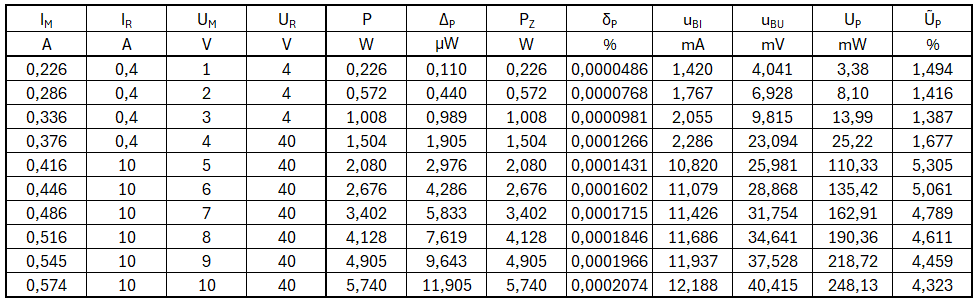
\includegraphics[width = \textwidth]{tabulka_av.png}
    \caption{Naměřené a vypočtené hodnoty - měření číslicovými přístroji v uspořádání \textbf{AV}}
\end{table}

\begin{table}[H]
    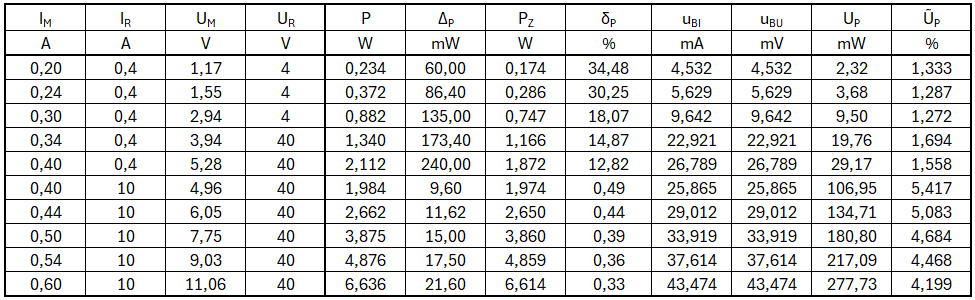
\includegraphics[width = \textwidth]{tabulka_va.png}
    \caption{Naměřené a vypočtené hodnoty - měření číslicovými přístroji v uspořádání \textbf{VA}}
\end{table}

\subsection{Grafy}

\begin{figure}[H]
    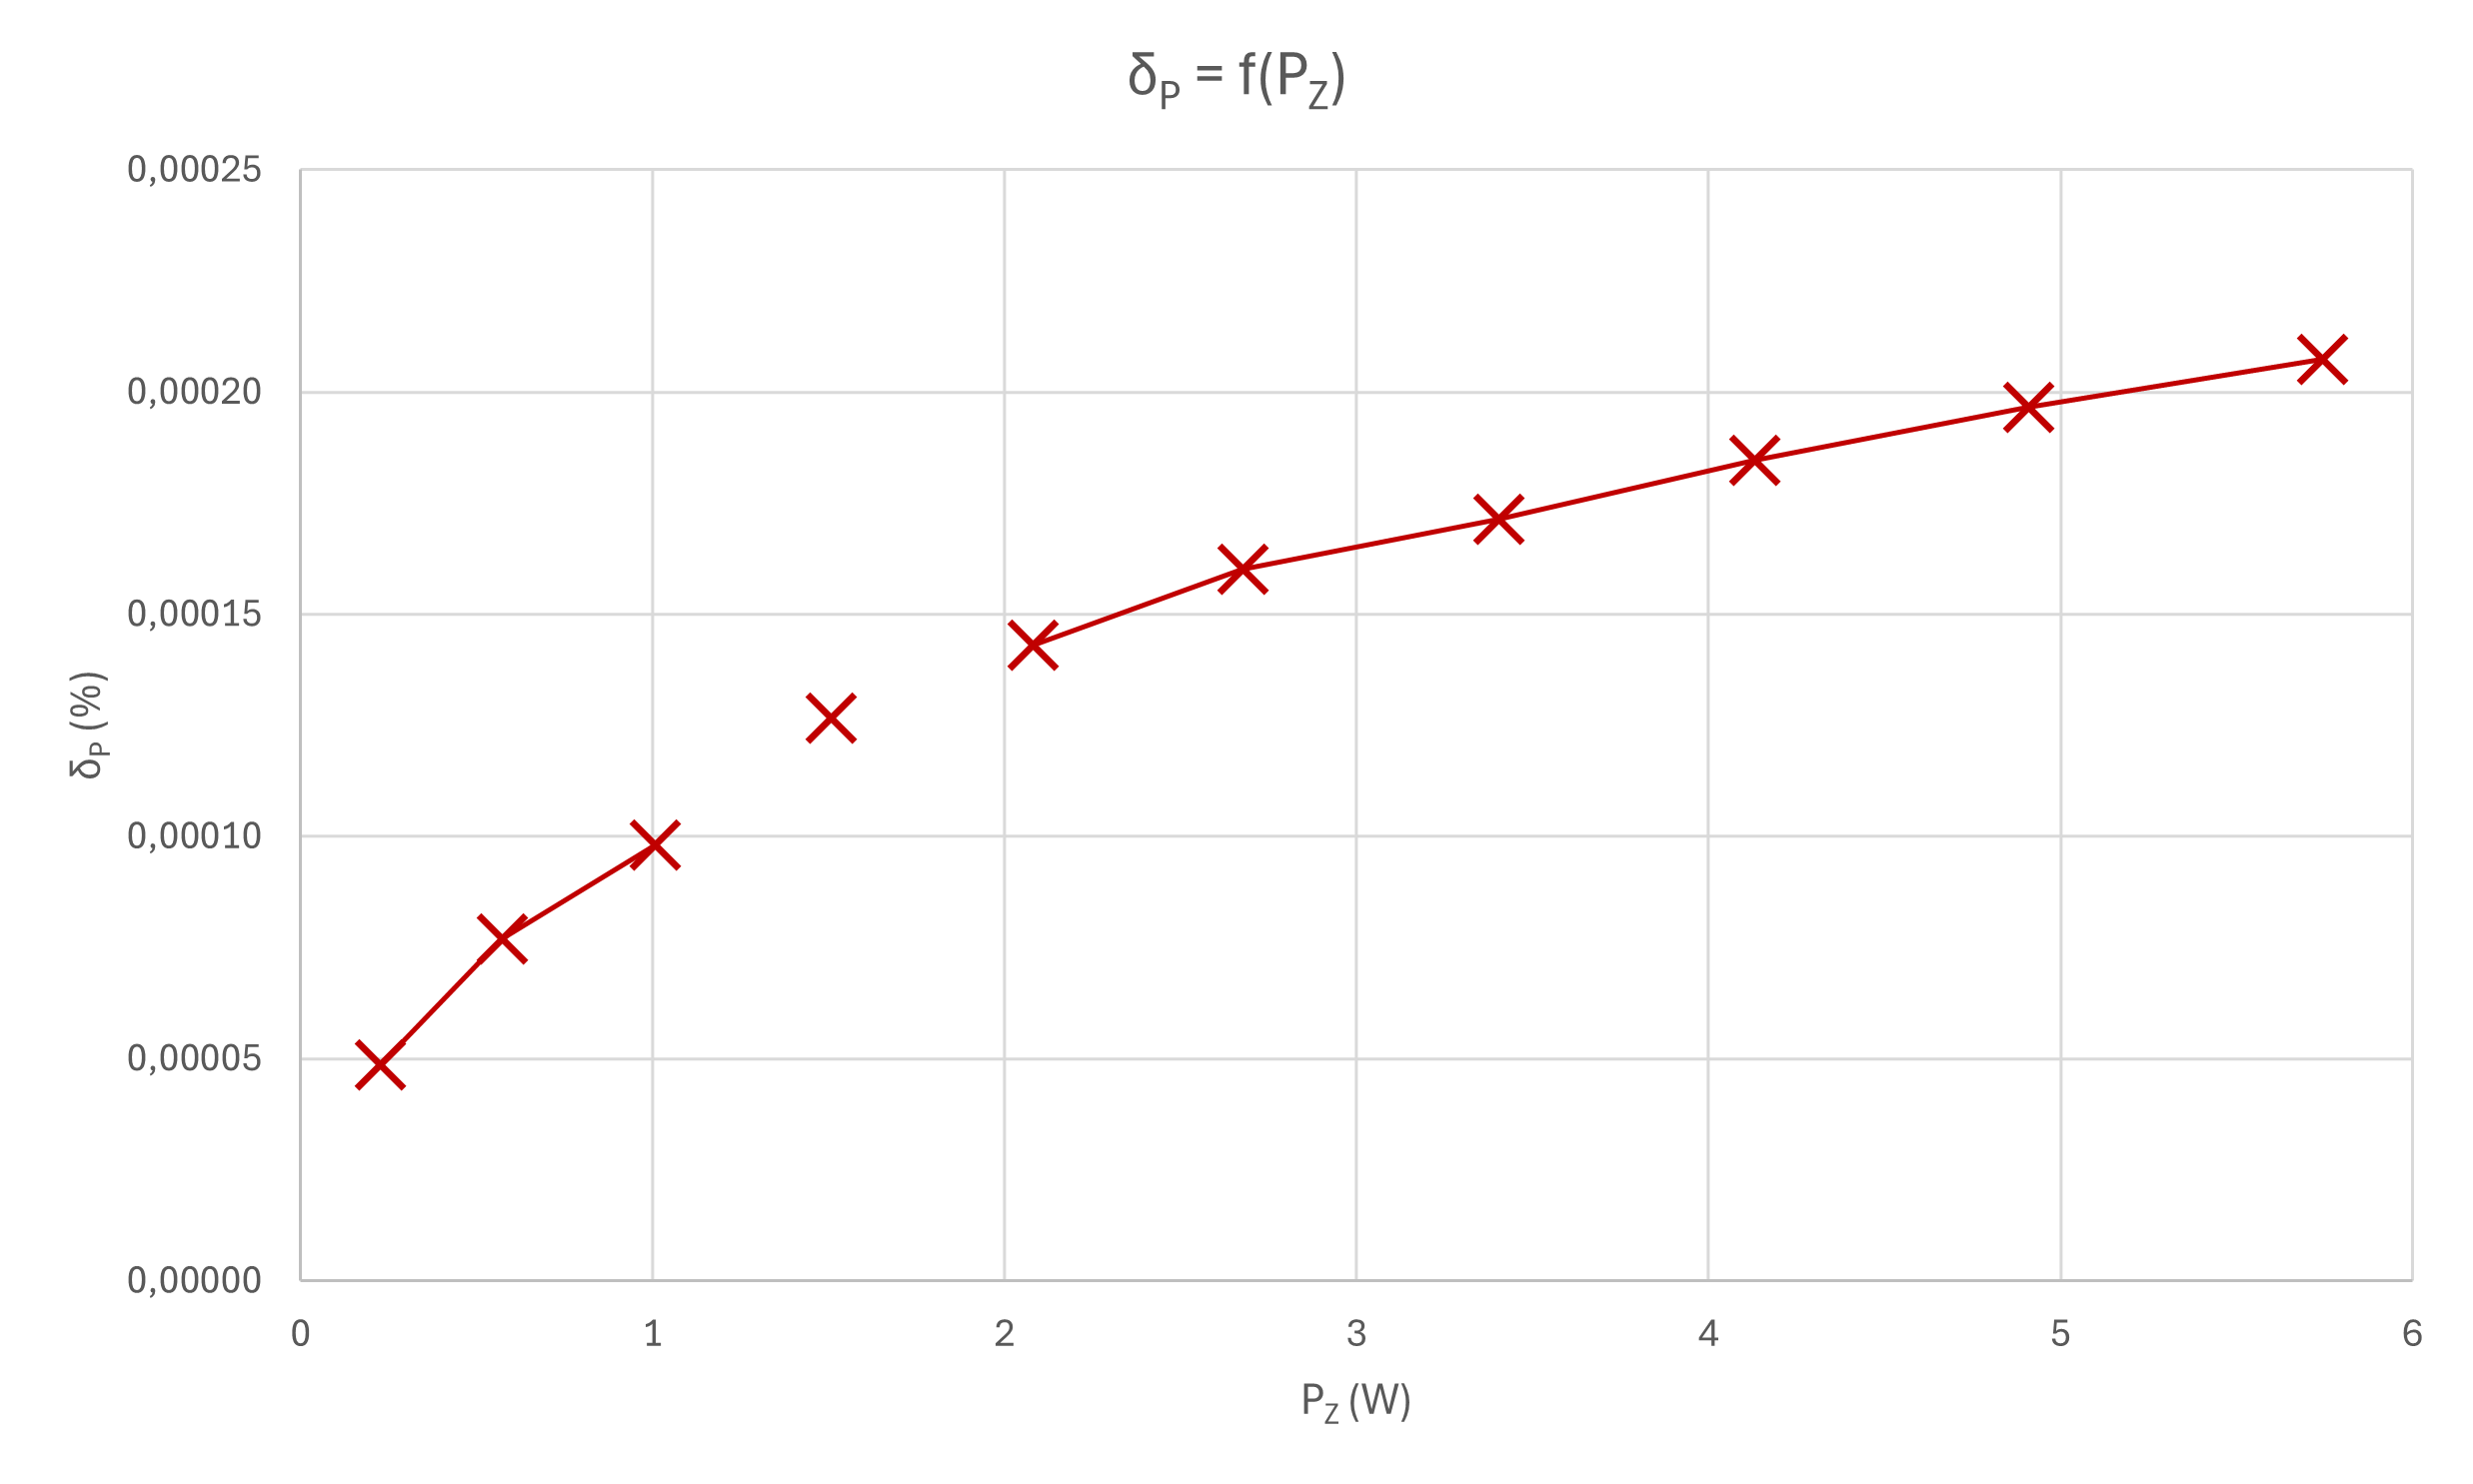
\includegraphics[width = \textwidth]{graf_av1.png}
    \caption{Graf závislosti relativní odchylky metody na výkonu zátěže v uspořádání \textbf{AV}}
\end{figure}

\begin{figure}[H]
    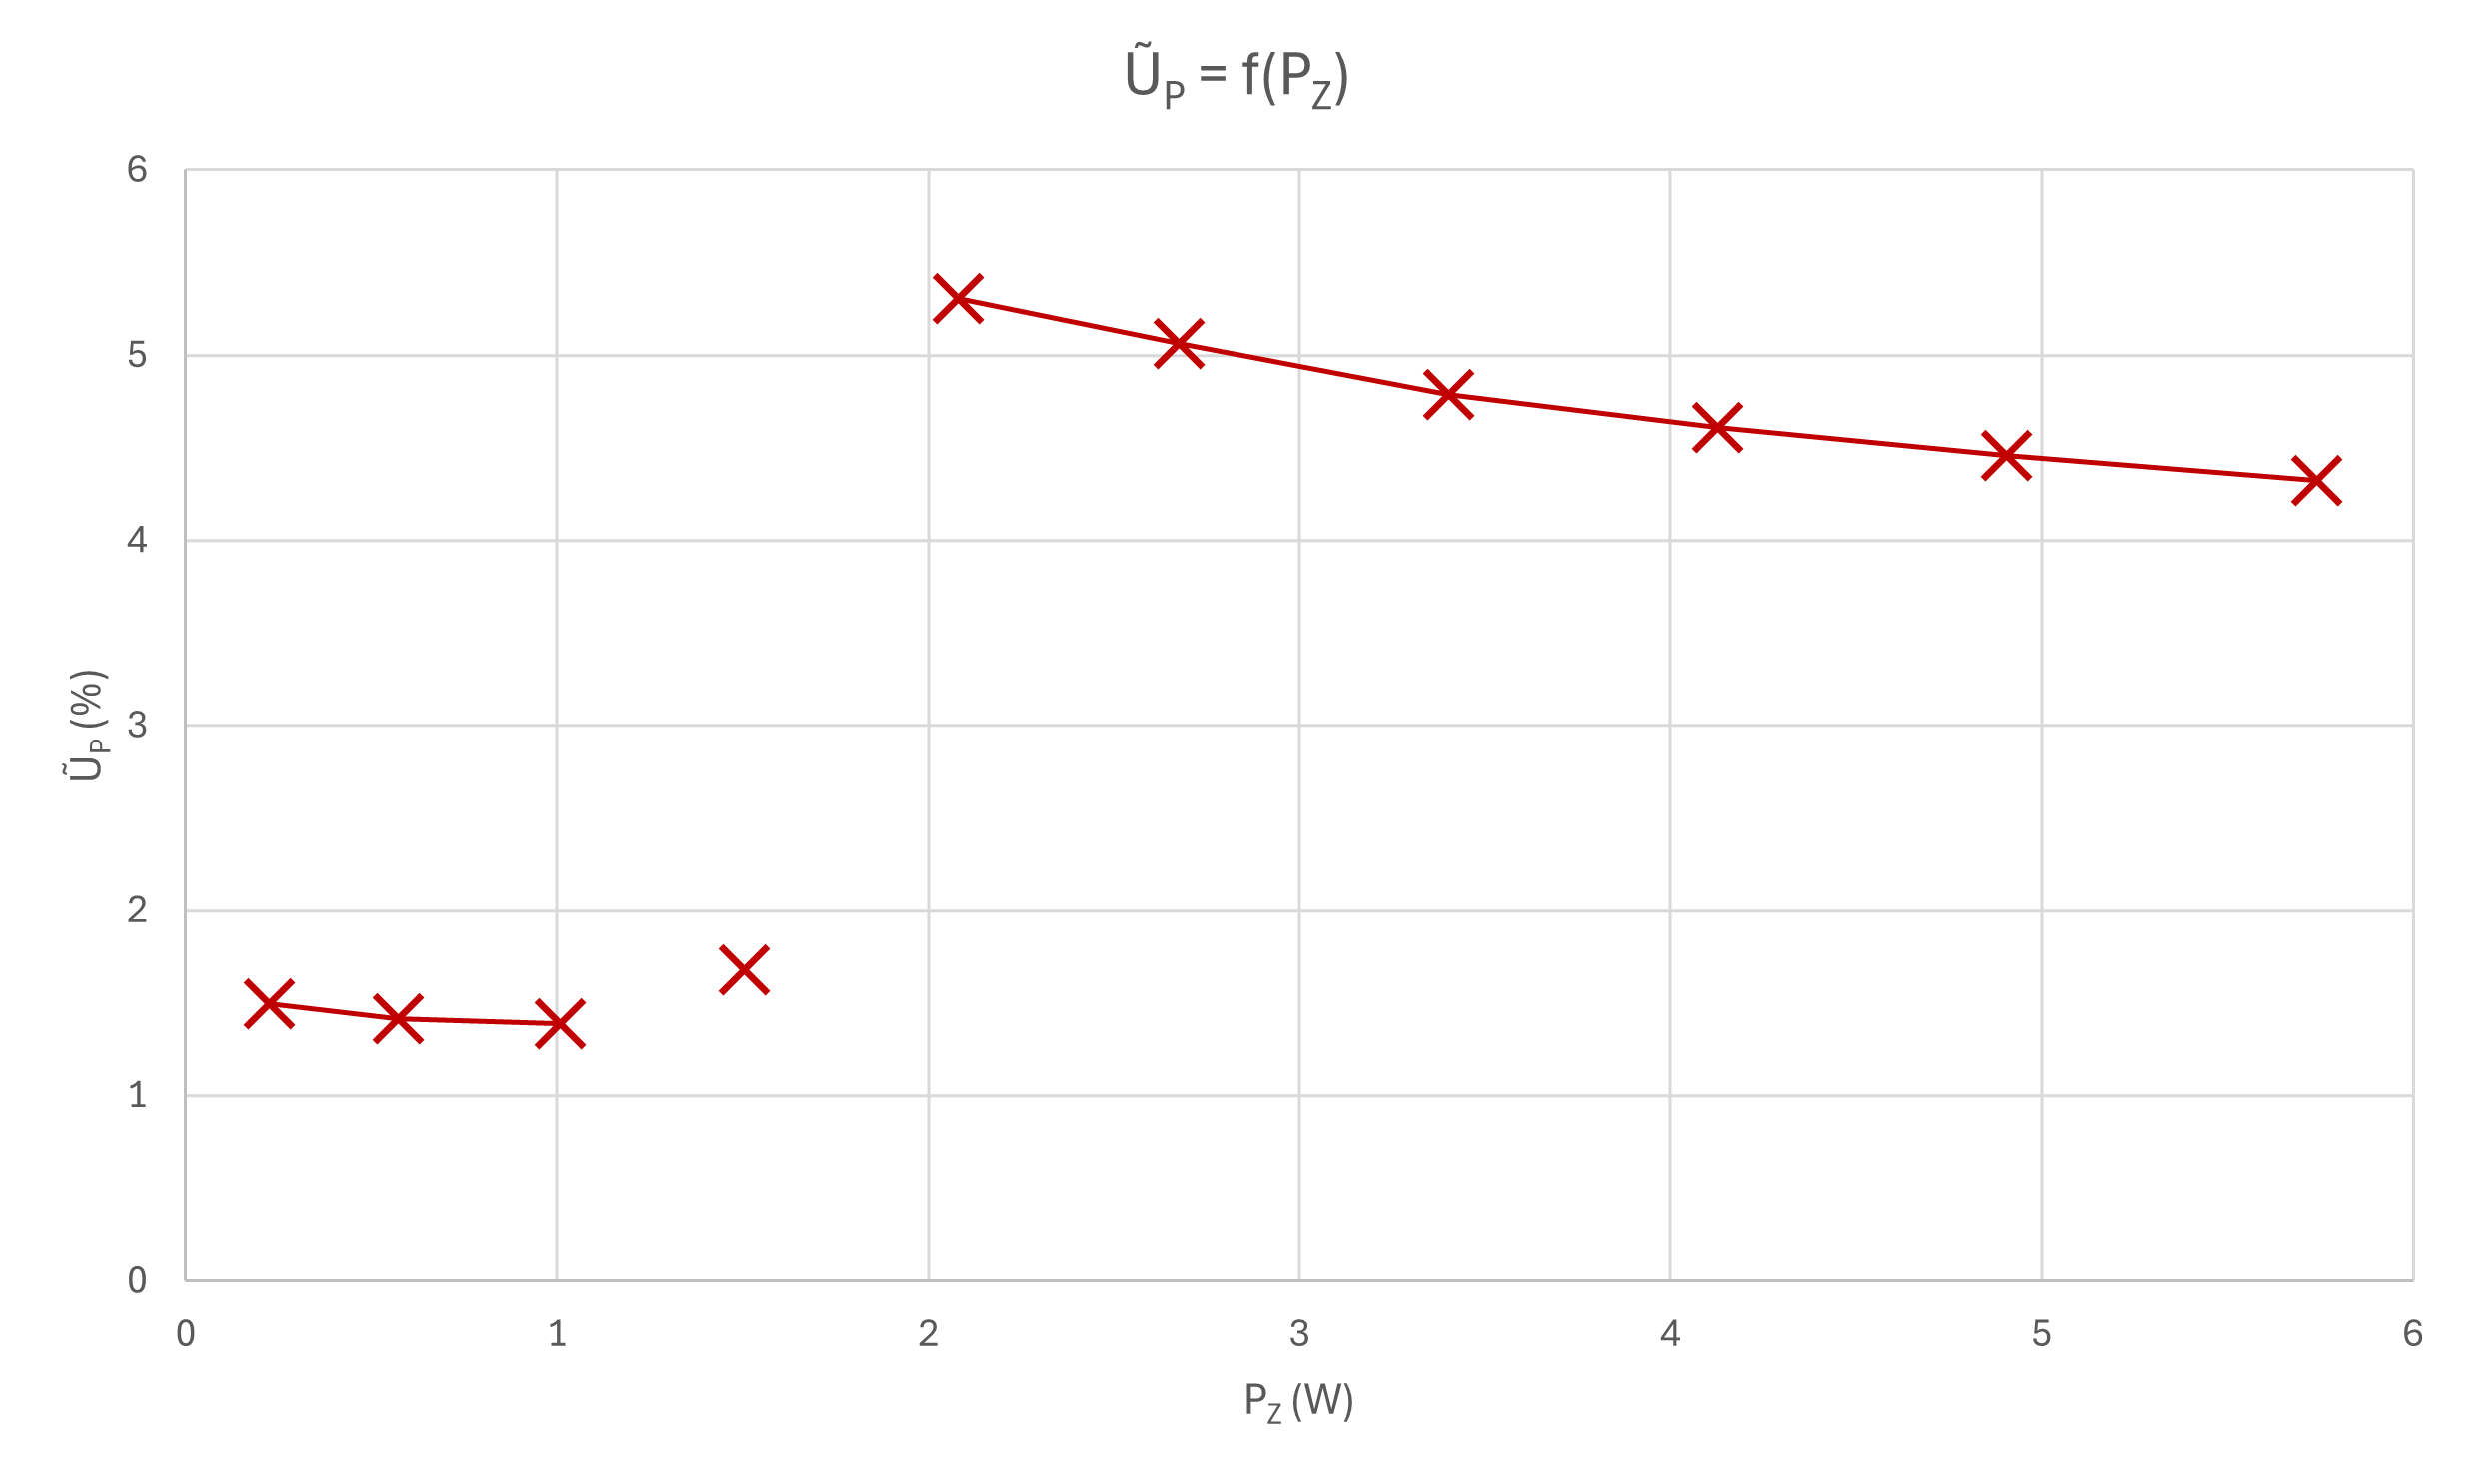
\includegraphics[width = \textwidth]{graf_av2.png}
    \caption{Graf závislosti relativní rozšířené nejistoty výsledků na výkonu zátěže v uspořádaní \textbf{AV}}
\end{figure}

\begin{figure}[H]
    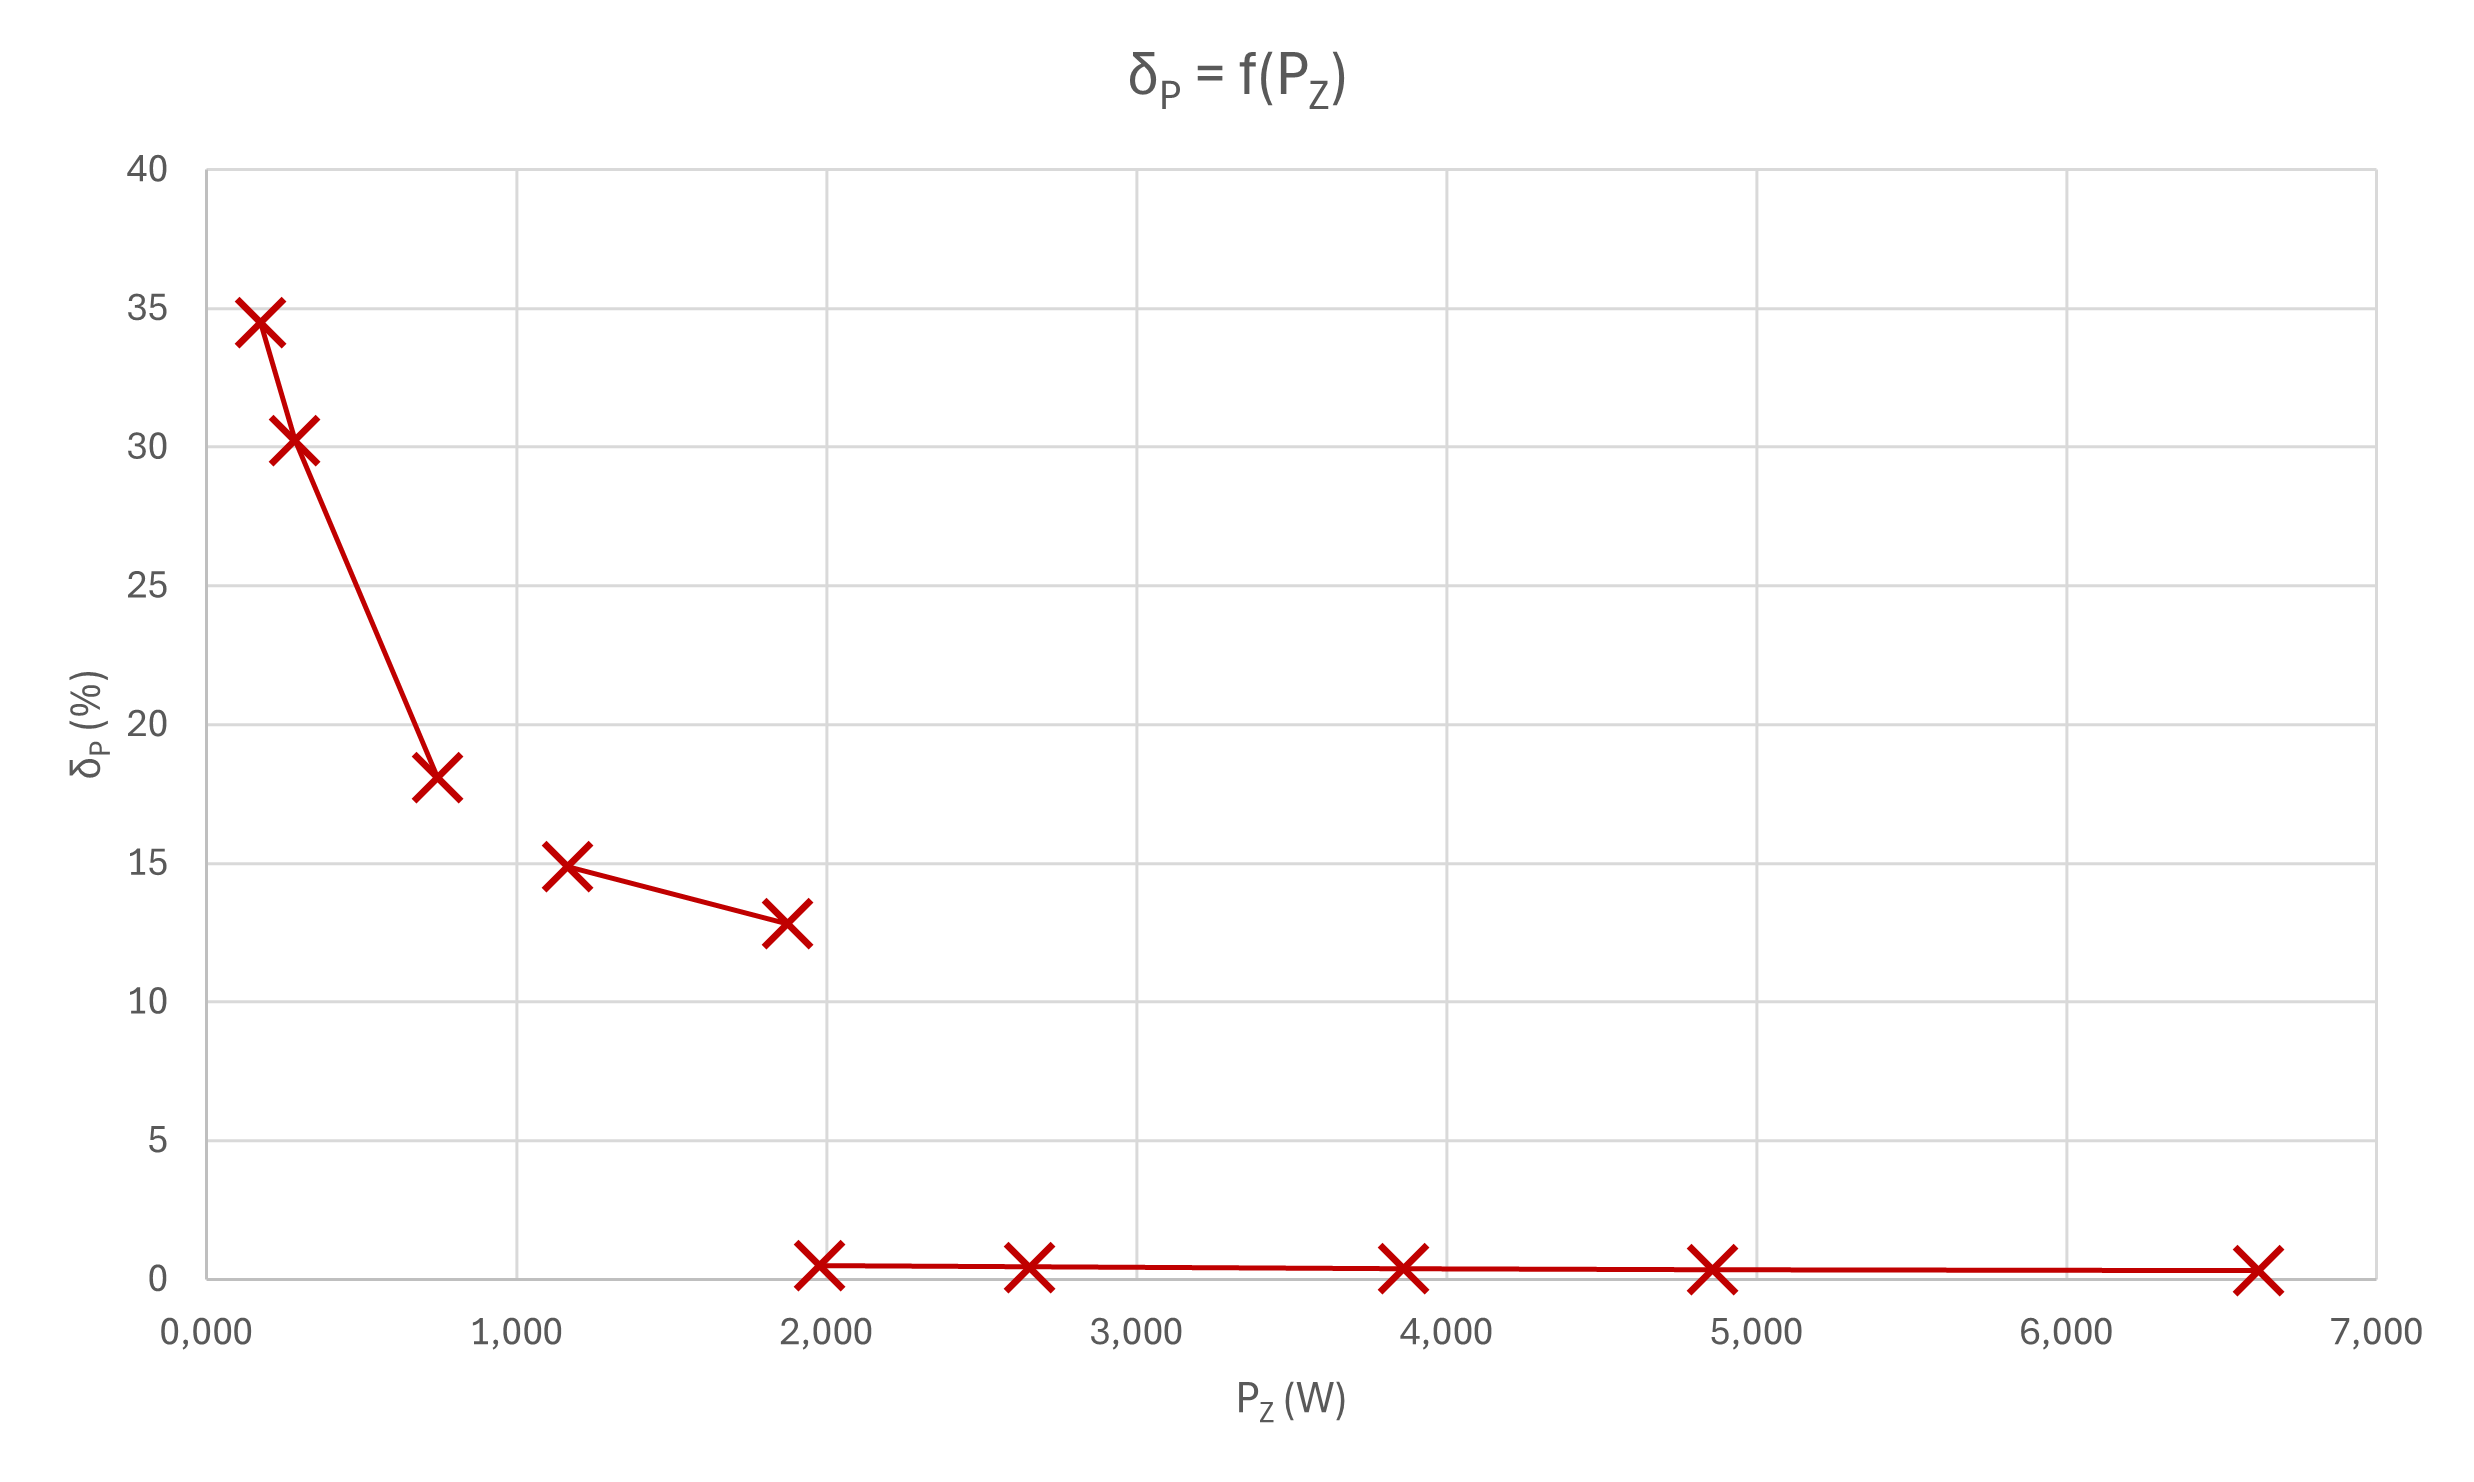
\includegraphics[width = \textwidth]{graf_va1.png}
    \caption{Graf závislosti relativní odchylky metody na výkonu zátěže v uspořádání \textbf{VA}}
\end{figure}

\begin{figure}[H]
    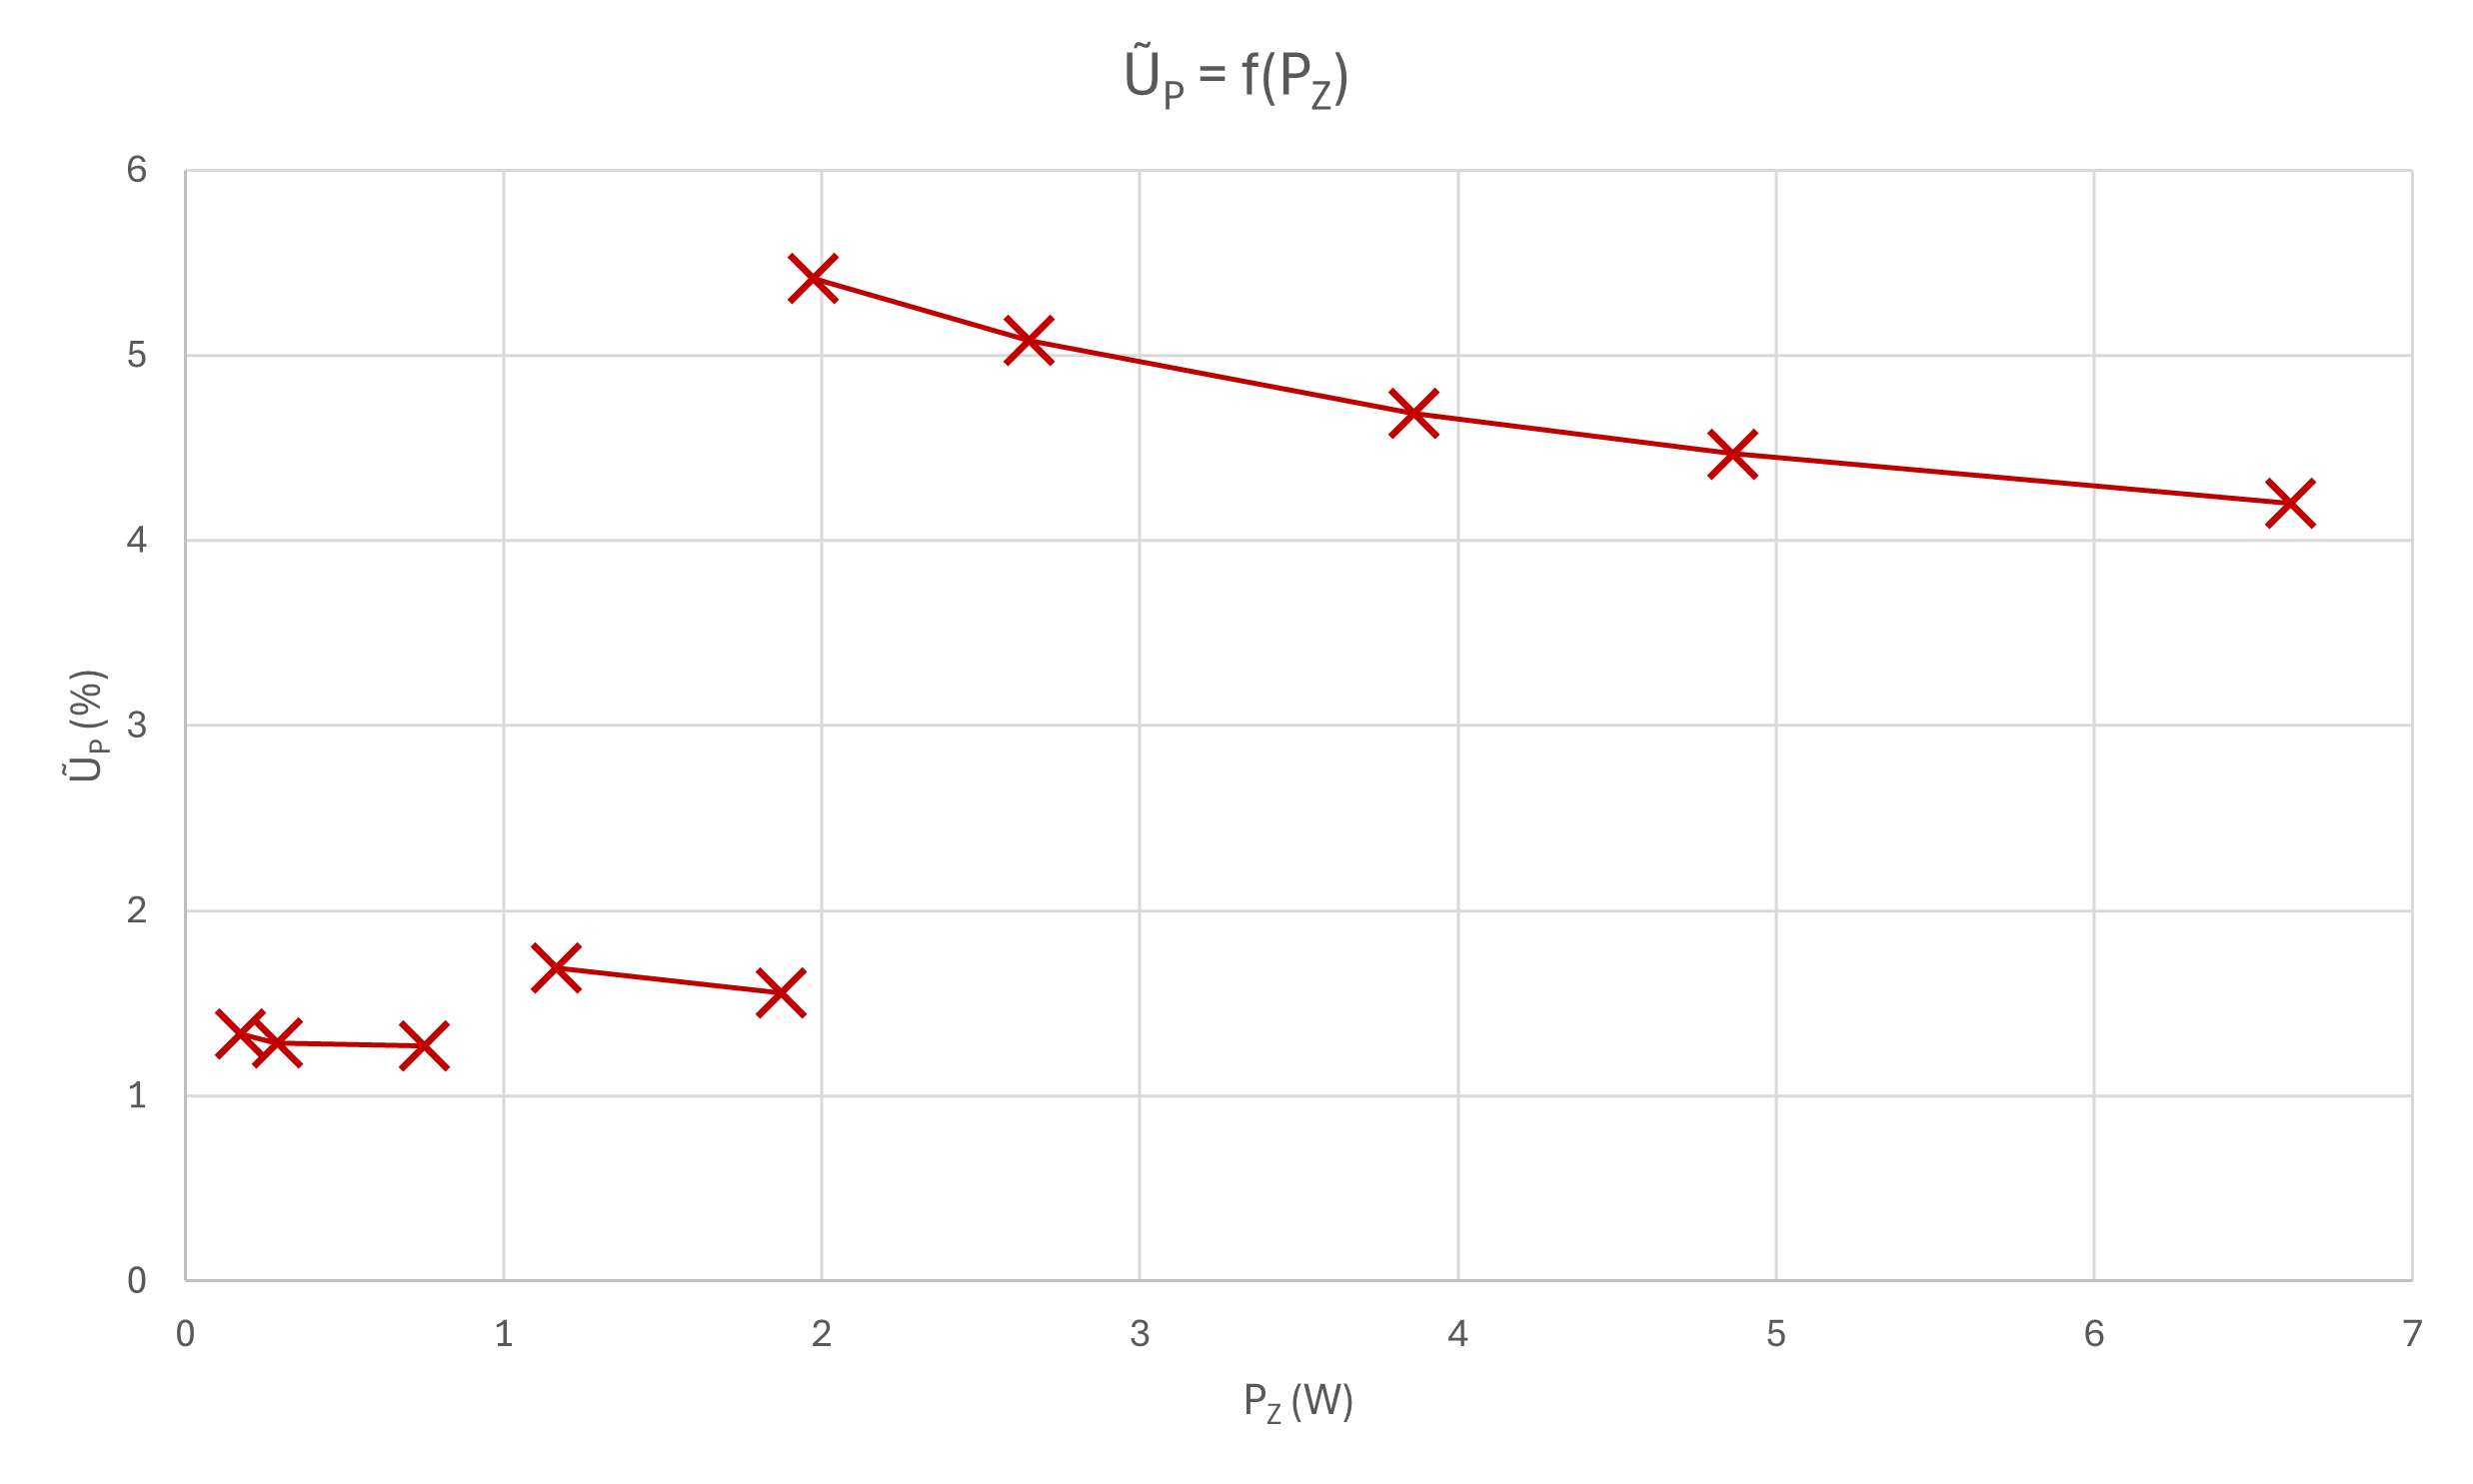
\includegraphics[width = \textwidth]{graf_va2.png}
    \caption{Graf závislosti relativní rozšířené nejistoty výsledků na výkonu zátěže v uspořádaní \textbf{VA}}
\end{figure}

\break

\subsection{Příklady výpočtů}

\begin{enumerate}
    \item Výkon (měřená veličina):
    \begin{multline*}
        P = \textcolor{teal}{U_V \cdot I_A} = U_M \cdot I_M = 1 V \cdot 0,226 A = \underline{\underline{0,266\ W}} \hfill
    \end{multline*}

    \item Absolutní odchylka metody:
    \begin{multline*}
        \Delta_{P_{AV}} = \textcolor{teal}{P_V = \frac{U_V^2}{R_V}} = \frac{U_M^2}{R_{V_{4V}}} = \frac{1^2 V}{9,1 \cdot 10^6 \Omega} = 109,89 \cdot 10^{-9} W = \underline{\underline{109,89\ nW}} \hfill
    \end{multline*}
    \begin{multline*}
        \Delta_{P_{VA}} = \textcolor{teal}{P_A = R_A \cdot I_A^2} = R_{A_{400mA}} \cdot I_M = 1,5 \Omega \cdot 0,2^2 A = 60 \cdot 10^{-3} W = \underline{\underline{60\ mW}} \hfill
    \end{multline*}

    \item Výkon zátěže:
    \begin{multline*}
        P_Z = \textcolor{teal}{P - \Delta_P} = 0,226 W - 109,89 \cdot 10^{-9} W = \underline{\underline{0,2259\ W}} \hfill
    \end{multline*}

    \item Relativní odchylka metody:
    \begin{multline*}
        \delta_P = \textcolor{teal}{\frac{\Delta_P}{P_Z} \cdot 100 \%} = \frac{109,89 \cdot 10^{-9} W}{0,2259 W} \cdot 100 \% = 48,62 \cdot 10^{-6} \% = \underline{\underline{0,000048623\ \%}} \hfill
    \end{multline*}

    \item Mezní odchylka měřícího rozsahu:
    \begin{multline*}
        \delta_{R_{A_{400mA}}} = \textcolor{teal}{\frac{d}{D} \cdot 100 \%} = \frac{2}{4000} \cdot 100 \% = \underline{\underline{0,05\ \%}} \hfill
    \end{multline*}

    \item Standardní přístrojová nejistota ČMP:
    \begin{multline*}
        u_{BI_{\Check{C}MP}} = \textcolor{teal}{\frac{\left| \delta_M \cdot X_M \right| + \left| \delta_R \cdot X_R \right|}{100 \cdot \chi}} = \frac{\left| \delta_{M_{A_{400mA}}} \cdot I_M \right| + \left| \delta_{R_{A_{400mA}}} \cdot I_R \right|}{100 \cdot \chi} = \frac{\left| 1 \% \cdot 0,226 A \right| + \left| 0,05 \% \cdot 0,4 A \right|}{100 \cdot \sqrt{3}} = \\
        = 1,420 \cdot 10^{-3} A = \underline{\underline{1,42\ mA}}
    \end{multline*}
    \begin{multline*}
        u_{BU_{\Check{C}MP}} = \textcolor{teal}{\frac{\left| \delta_{M_{V}} \cdot U_M \right| + \left| \delta_{R_{V}} \cdot U_R \right|}{100 \cdot \chi}} = \frac{|0,5 \% \cdot 1 V|+|0,05 \% \cdot 4 V|}{100 \cdot \sqrt{3}} = 4,041 \cdot 10^{-3}\ V = \underline{\underline{4,041\ mV}} \hfill
    \end{multline*}

    \item Standardní nejistota výsledku:
    \begin{multline*}
        u_{P_{AV}} = \textcolor{teal}{\sqrt{\left( \left( I_A - \frac{2 \cdot U_V}{R_V} \right) \cdot u_{BU} \right)^2 + \left( U_V \cdot u_{BI} \right)^2}} = \sqrt{\left( \left( I_M - \frac{2 \cdot U_M}{R_{V_{4V}}} \right) \cdot u_{BU_{\Check{C}MP}} \right)^2 + \left( U_M \cdot u_{BI_{\Check{C}MP}} \right)^2} = \\
        = \sqrt{\left( \left( 0,266A - \frac{2 \cdot 1V}{9,1 \cdot 10^6 \Omega} \cdot 4,041 \cdot 10^{-3}V \right) \right)^2 + \left( 1V \cdot 1,42 \cdot 10^{-3}A \right)^2} = 1,688 \cdot^{-3}W = \underline{\underline{1,688\ mW}}
    \end{multline*}
    \begin{multline*}
        u_{P_{VA}} = \textcolor{teal}{\sqrt{\left( I_A \cdot u_{BU} \right)^2 + \left( \left( U_V - 2 \cdot R_A \cdot I_A \right) \cdot u_{BI} \right)^2}} = \sqrt{\left( I_M \cdot u_{BU_{\Check{C}MP}} \right)^2 + \left( \left( U_M - 2 \cdot R_{A_{400mA}} \cdot I_M \right) \cdot u_{BI_{\Check{C}MP}} \right)^2} =  \\
        = \sqrt{\left( 0,2A \cdot 4,532 \cdot 10^{-3}V \right)^2 + \left( \left( 1,17V - 2 \cdot 1,5 \Omega \cdot 0,2A \right) \cdot 1,27 \cdot 10^{-3}A \right)^2} = 1,16 \cdot 10^{-3} W = \underline{\underline{1,16\ mW}}
    \end{multline*}

    \item Rozšířená nejistota:
    \begin{multline*}
        U_P = \textcolor{teal}{u_p \cdot k_r} = u_{P_{AV}} \cdot k_r = 1,688 \cdot 10^{-3} W \cdot 2 = 3,376 \cdot 10^{-3} W = \underline{\underline{3,376\ mW}} \hfill
    \end{multline*}

    \item Relativní rozšířená nejistota:
    \begin{multline*}
        \tilde{U}_P = \textcolor{teal}{\frac{U_P}{Y_{kor}} \cdot 100 \%} = \frac{U_P}{P_Z} \cdot 100 \% = \frac{3,376 \cdot 10^{-3} W}{0,2259 W} \cdot 100 \% = \underline{\underline{1,49\ \%}} \hfill
    \end{multline*}
\end{enumerate}

\section{Seznam použitých přístrojů}

\begin{itemize}
    \item Číslicový multimetr Finest 703 TRUE RMS, v.č. 180601917
    \item Číslicový multimetr Finest 703 TRUE RMS, v.č. 180601995
    \item Jednosměrný zdroj Keysight U8001A, v.č. MY58170017
\end{itemize}

\section{Závěr}

Z naměřených a vypočtených závislostí je patrné, že relativní odchylka metody $\delta_P$ v případě AV uspořádání zapojení stoupá a v případě VA uspořádání naopak klesá.
Relativní nejistota měření má tendenci klesat, no při vyšších měřících rozsazích výrazně skokově stoupá.

Pro měření výkonu na malých odporových zátěžích se zdá být vhodnější použít uspořádání AV, kde je odchylka metody řádově nižší než při použití uspořádání VA, kde se projevuje velká odchylka způsobená úbytkem napětí na ampérmetru.
Pro velké odporové zátěže je naopak vhodné použít uspořádání VA z důvodu dělení proudu do obvodové větve voltmetru.

\end{document}